\chapter{Projekt i Struktura Bazy Danych}
\label{chap:baza_danych}

Fundamentem aplikacji jest relacyjna baza danych o nazwie \texttt{szosp}, która została zaprojektowana w celu przechowywania i zarządzania wszystkimi informacjami dotyczącymi strażaków, pojazdów, interwencji oraz użytkowników systemu. Baza danych składa się z czterech głównych tabel oraz dwóch tabel łączących, które realizują relacje wiele-do-wielu. Schemat bazy danych został przedstawiony na diagramie encji-związków (Rys. \ref{fig:erd}).

\begin{figure}[H]
	\centering
	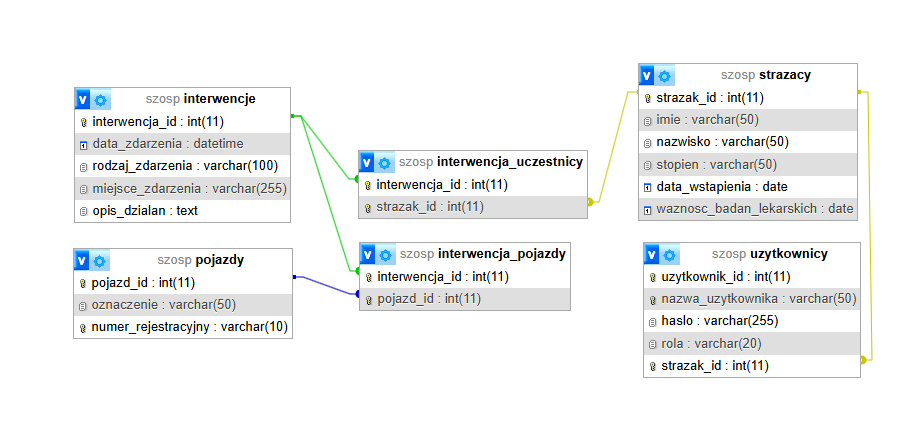
\includegraphics[width=\textwidth]{figures/BazaDanych.png}
	\caption{Diagram encji-związków (ERD) dla bazy danych \texttt{szosp}.}
	\label{fig:erd}
\end{figure}

\section{Opis Tabel}
\label{sec:opis_tabel}

Poniżej przedstawiono szczegółowy opis poszczególnych tabel wchodzących w skład bazy danych.

\subsection{Tabela \texttt{strazacy}}
Tabela ta przechowuje podstawowe dane osobowe oraz służbowe każdego strażaka.
\begin{itemize}
    \item \texttt{strazak\_id}: Klucz główny, unikalny identyfikator strażaka (INT).
    \item \texttt{imie}: Imię strażaka (VARCHAR(50)).
    \item \texttt{nazwisko}: Nazwisko strażaka (VARCHAR(50)).
    \item \texttt{stopien}: Stopień służbowy (VARCHAR(50)).
    \item \texttt{data\_wstapienia}: Data wstąpienia do służby (DATE).
    \item \texttt{waznosc\_badan\_lekarskich}: Data ważności badań lekarskich (DATE).
\end{itemize}

\subsection{Tabela \texttt{uzytkownicy}}
Tabela odpowiedzialna za przechowywanie danych logowania i uprawnień użytkowników systemu.
\begin{itemize}
    \item \texttt{uzytkownik\_id}: Klucz główny, unikalny identyfikator użytkownika (INT).
    \item \texttt{nazwa\_uzytkownika}: Login użytkownika (VARCHAR(50)).
    \item \texttt{haslo}: Hasło użytkownika, przechowywane jako skrót (VARCHAR(255)).
    \item \texttt{rola}: Rola użytkownika w systemie, np. admin (VARCHAR(20)).
    \item \texttt{strazak\_id}: Klucz obcy wskazujący na powiązanego strażaka (INT).
\end{itemize}

\subsection{Tabela \texttt{pojazdy}}
Ewidencja pojazdów będących na wyposażeniu jednostki.
\begin{itemize}
    \item \texttt{pojazd\_id}: Klucz główny, unikalny identyfikator pojazdu (INT).
    \item \texttt{oznaczenie}: Oznaczenie taktyczne pojazdu (VARCHAR(50)).
    \item \texttt{numer\_rejestracyjny}: Numer rejestracyjny pojazdu (VARCHAR(10)).
\end{itemize}

\subsection{Tabela \texttt{interwencje}}
Główna tabela przechowująca informacje o przeprowadzonych interwencjach.
\begin{itemize}
    \item \texttt{interwencja\_id}: Klucz główny, unikalny identyfikator interwencji (INT).
    \item \texttt{data\_zdarzenia}: Dokładna data i czas zdarzenia (DATETIME).
    \item \texttt{rodzaj\_zdarzenia}: Kategoria zdarzenia (VARCHAR(100)).
    \item \texttt{miejsce\_zdarzenia}: Adres/lokalizacja zdarzenia (VARCHAR(255)).
    \item \texttt{opis\_dzialan}: Szczegółowy opis podjętych działań (TEXT).
\end{itemize}

\subsection{Tabele Łączące}
W celu zrealizowania relacji wiele-do-wielu, w projekcie wykorzystano dwie tabele pośredniczące.
\begin{itemize}
    \item \texttt{interwencja\_uczestnicy}: Tabela łącząca interwencje ze strażakami, którzy brali w nich udział. Składa się z dwóch kluczy obcych: \texttt{interwencja\_id} oraz \texttt{strazak\_id}.
    \item \texttt{interwencja\_pojazdy}: Tabela łącząca interwencje z pojazdami, które były do nich zadysponowane. Składa się z dwóch kluczy obcych: \texttt{interwencja\_id} oraz \texttt{pojazd\_id}.
\end{itemize}

\section{Relacje Między Tabelami}
\label{sec:relacje_tabel}

Diagram ERD (Rys. \ref{fig:erd}) ilustruje kluczowe powiązania między tabelami.
\begin{itemize}
    \item \textbf{Relacja jeden-do-jednego} występuje między tabelami \texttt{strazacy} a \texttt{uzytkownicy}. Każdy strażak może mieć dokładnie jedno konto użytkownika w systemie, a każde konto jest przypisane do jednego strażaka. Relacja ta jest realizowana poprzez klucz obcy \texttt{strazak\_id} w tabeli \texttt{uzytkownicy}.
    \item \textbf{Relacja wiele-do-wielu} łączy tabelę \texttt{interwencje} z tabelą \texttt{strazacy} za pośrednictwem tabeli \texttt{interwencja\_uczestnicy}. Pozwala to na przypisanie wielu strażaków do jednej interwencji oraz na udział jednego strażaka w wielu różnych interwencjach.
    \item \textbf{Relacja wiele-do-wielu} łączy również tabelę \texttt{interwencje} z tabelą \texttt{pojazdy} za pomocą tabeli \texttt{interwencja\_pojazdy}. Dzięki temu do jednej interwencji można przypisać wiele pojazdów, a jeden pojazd może być wykorzystywany w wielu akcjach.
\end{itemize}